\chapter{Rings}\label{chap:rings}
\begin{summary}
\item Ring, commutative ring, divison ring, field. Subring, subring criterion. Zero divisors, integral domains. Units. Characteristic of ring. Fields of fractions and their characterisation.
\item Homomorphisms of rings. Quotient rings, ideals and the first isomorphism theorem and consequences, e.g. Chinese remainder theorem. Relation between ideals in $R$ and $R/I$. Prime ideals and maximal ideals, relation to fields and integral domains. Application of quotients to constructing fields by adjunction of elements. Degree of a field extension, the tower law.
\item Euclidean domains. Principal ideal domains. EDs are PIDs. Unique factorisation for PIDs. Gauss's lemma and Eisenstein's criterion for irreducibility.
\item Polynomial rings.
\end{summary}

\section{Rings}
\begin{definition}[Ring]
A \vocab{ring}\index{ring} $(R,+,\times,0,1)$ consists of a set $R$, $0,1\in R$, together with two binary operations addition and multiplication, denoted $+$ and $\times$, satisfying the following axioms:
\begin{enumerate}[label=(\roman*)]
\item $(R,+)$ is an abelian group with additive identity $0$.
\item $\times$ is associative, with multiplicative identity $1$.
\item $\times$ distributes over $+$: for all $a,b,c\in R$,
\begin{align*}
a\times(b+c)&=(a\times b)+(a\times c),\\
(a+b)\times c&=(a\times c)+(b\times c).
\end{align*}
\end{enumerate}
\end{definition}

\begin{notation}
We simply write $ab$ rather than $a\times b$ for $a,b\in R$.
\end{notation}

$R$ is a \vocab{commutative ring} if $\times$ is commutative.

\begin{definition}
A ring $R$ with identity $1$, where $1\neq0$, is called a \vocab{division ring}\index{ring!division ring} if every $a\in R\setminus\{0\}$ has a multiplicative inverse, i.e. exists $b\in R$ such that $ab=ba=1$.

A commutative division ring is called a \vocab{field}\index{ring!field}.
\end{definition}

\begin{figure}[H]
\centering
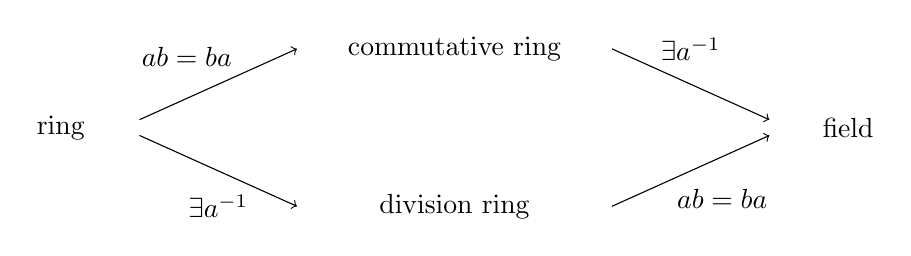
\begin{tikzpicture}
\node at (-0.5,0) {ring};
\draw[->] (0.5,0.1) -- (2.5,1);
\node at (1.1,0.9) {$ab=ba$};
\node at (4.5,1) {commutative ring};
\draw[->] (0.5,-0.1) -- (2.5,-1);
\node at (1.5,-1) {$\exists a^{-1}$};
\node at (4.5,-1) {division ring};
\draw[->] (6.5,1) -- (8.5,0.1);
\node at (7.5,1) {$\exists a^{-1}$};
\draw[->] (6.5,-1) -- (8.5,-0.1);
\node at (7.9,-0.9) {$ab=ba$};
\node at (9.5,0) {field};
\end{tikzpicture}
\end{figure}

\begin{example}
$\ZZ$ under usual addition and multiplication is a commutative ring with identity $1$.

$\QQ$, $\RR$, $\CC$ are fields.

$\ZZ_n$ is a commutative ring with identity $\bar{1}$ under addition and multiplication of residue classes.
\end{example}

\begin{proposition}
Let $R$ be a ring. Then
\begin{enumerate}[label=(\roman*)]
\item $0a=a0=0$ for all $a\in R$.
\item $(-a)b=a(-b)=-(ab)$ for all $a,b\in R$.
\item $(-a)(-b)=ab$ for all $a,b\in R$.
\item if $R$ has identity $1$, then the identity is unique and $-a=(-1)a$.
\end{enumerate}
\end{proposition}

\begin{proof}
These all follow from the distributive laws and cancellation in the additive group $(R,+)$.
\begin{enumerate}[label=(\roman*)]
\item $0a=(0+0)a=0a+0a$ then add the additive identity of $0a$ to both sides to get $0a=0$. Similarly, $a0=a(0+0)=a0+a0$ then add the additive identity of $a0$ to both sides to get $a0=0$.
\item 
\item 
\item 
\end{enumerate}
\end{proof}

\begin{definition}[Subring]
$S\subset R$ is a \vocab{subring}\index{ring!subring} of ring $R$ if $S$ is a subgroup of $R$ that is closed under multiplication.
\end{definition}

If $R$ contains $1$, then $S$ is a (unital) subring if $1_R\in S$. We assume subrings are unital unless otherwise specified.

\begin{lemma}[Subring criterion]
Let $R$ be a ring, $S\subset R$. Then $S$ is a subring of $R$ if and only if
\begin{enumerate}[label=(\roman*)]
\item $1\in S$;
\item $s_1s_2\in S$ and $s_1-s2\in S$ for all $s_1,s_2\in S$.
\end{enumerate}
\end{lemma}

\begin{proof} \

\fbox{$\implies$}

\fbox{$\impliedby$} The condition that $s_1-s_2\in S$ for all $s_1,s_2\in S$ implies that $S$ is an additive subgroup by the subgroup test (note that as $1\in S$ we know that $S$ is nonempty). The other conditions for a subring hold directly.
\end{proof}

Recall that in a ring we do not require that nonzero elements have a multiplicative inverse. Nevertheless, because the multiplication operation is associative and there is a multiplicative identity, the elements which happen to have multiplicative inverses form a group:

\begin{definition}[Unit]
Let $R$ be a ring. $a\in R$ is called a \vocab{unit} in $R$ if there exists $b\in R$ such that $ab=ba=1$.
\end{definition}

\begin{proposition}
The units in a ring $R$ form a group under multiplication.
\end{proposition}

\begin{definition}[Group of units]
Let $R$ be a ring. The subset
\[R^\times = \{r\in R\mid \exists s\in R, rs=1\}\]
is called the \vocab{group of units} in $R$; it is a group under multiplication $\times$ with identity element $1$.
\end{definition}

\begin{definition}
Let $R$ be a ring. $a\in R\setminus\{0\}$ is called a \vocab{zero divisor}\index{zero divisor} if there exists $b\in R\setminus\{0\}$ such that either $ab=0$ or $ba=0$.

A ring which is not the zero ring and has no zero divisors is called an \vocab{integral domain}\index{integral domain}. Thus if a ring is an integral domain and a.b = 0 then one of a or b is equal to zero.
\end{definition}

The absence of zero divisors in integral domains give these rings a cancellation property:

\begin{proposition}
Let $R$ be a ring. $a,b,c\in R$, $a$ is not a zero divisor. If $ab=ac$, then either $a=0$ or $b=c$. In particular, for any $a,b,c$ in an integral domain and $ab=ac$, then either $a=0$ or $b=c$.
\end{proposition}

\begin{proof}
If $ab=ac$ then $a(b-c)=0$ so either $a=0$ or $b-c=0$. The second statement follows from the definition of an integral domain.
\end{proof}

\begin{corollary}
Any finite integral domain is a field.
\end{corollary}

\begin{proposition}
$\ZZ_p$ is a field if and only if $p$ is prime. If $p$ is composite, then there exists a zero divisor.
\end{proposition}

\begin{remark}
Fields $\subset$ integral domains $\subset$ commutative unital rings.
\end{remark}

\begin{definition}
Let $R$ be a ring, if for all $a\in R$, there exists $m\in\ZZ^+$ such that $ma=0$, then R is called a ring of \emph{finite characteristic}.
\end{definition}

\begin{definition}[Characterisitc]
The \vocab{characterisitc} of a ring $R$ is the smallest number of times one must add $1_R$ to get $0_R$.
\end{definition}

\section{Ring Homomorphisms and Ideals}
From now on we will assume all our rings are commutative.

\begin{definition}
$\phi:R\to S$ is a \vocab{homomorphism}\index{homomorphism} if it satisfies
\begin{enumerate}[label=(\roman*)]
\item $\phi(1_R)=1_S$;
\item $\phi(r_1+r_2)=\phi(r_1)+\phi(r_2)$ for all $r_1,r_2\in R$;
\item $\phi(r_1r_2)=\phi(r_1)\phi(r_2)$ for all $r_1,r_2\in R$.
\end{enumerate}
A bijective ring homomorphism is called an \vocab{isomorphism}\index{isomorphism}, denoted by $R\cong S$.
\end{definition}

\begin{definition}
Let $\phi:R\to S$ be a homomorphism. The \vocab{kernel} of $\phi$ is
\[\ker\phi\coloneqq\{r\in R\mid\phi(r)=0\},\]
and the \vocab{image} of $\phi$ is
\[\im\phi\coloneqq\{s\in S\mid \exists r\in R, \phi(r)=s\}.\]
If $\im\phi=S$, we say that $\phi$ is surjective.
\end{definition}

\begin{definition}
Let $R$ be a ring, $I\subset R$, and let $r\in R$. Write
\begin{align*}
rI&=\{ra\mid a\in I\}\\
Ir&=\{ar\mid a\in I\}
\end{align*}
$I\subset R$ is a \emph{left ideal} of $R$ if
\begin{enumerate}[label=(\roman*)]
\item $I$ is a subring of $R$;
\item $I$ is closed under left multiplication by elements of $R$.
\end{enumerate}
(A right ideal is similarly defined [closed under right multiplication]).

$I\subset R$ that is both a left and right ideal is called an \vocab{ideal} of $R$.
\end{definition}

For commutative rings, left, right and ideals coincide.

\begin{lemma}
If $\phi:R\to S$ is a ring homomorphism, then $\ker\phi$ is an ideal. Moreover $I\subset R$ is an ideal if and only if it is nonempty, closed under addition, and closed under multiplication by arbitrary elements of $R$.
\end{lemma}

\begin{proof}
This is immediate from the definitions. For the moreover part, we just need to check that $I$ is closed under taking additive inverses. But this follows from the fact that it is closed under multiplication by any element of $R$ since $-x=(-1)x$ for any $x\in R$.
\end{proof}

Note that if $I$ is an ideal of $R$ which contains $1$, then $I=R$. We will shortly see that in fact any ideal is the kernel of a homomorphism. First let us note a few basic properties of ideals:



\begin{definition}
Let $I\subset R$ be an ideal. Then the quotient ring is
\[R/I\coloneqq\{x+I\mid x\in R\}.\]
\end{definition}

\begin{lemma}
$R/I$ is a ring, with addition and multiplication defined as
\begin{align*}
(x+I)+(y+I)&=(x+y)+I,\\
(x+I)\cdot(y+I)&=xy+I.
\end{align*}
\end{lemma}



\section{Chinese Remainder Theorem}
\section{Prime and Maximal Ideals}
Let $R$ be a commutative ring.

\begin{definition}
An ideal $P\subset R$ is called \vocab{prime} if $xy\in P$ implies either $x\in P$ or $y\in P$.

An ideal $M\subset R$ is called \vocab{maximal} if there is no ideal between $M$ and $R$, i.e., for ideal $U$ in $R$ and $M\subset U\subset R$ implies $U=M$.
\end{definition}

\begin{example}
Every ideal in $\ZZ$ is of the form $n\ZZ$ for $n\in\ZZ$. Then $p\ZZ$ for $p$ prime is a prime ideal and, notably, $\{0\}$ is a prime ideal. Further $p\ZZ\subset U=n\ZZ\subset\ZZ$, and $p\in U$, then $p=nq$ for some $q\in\ZZ$. But $p$ is prime and $n\neq1$ so $n=p$. Thus $U=p\ZZ$. Thus $p\ZZ$, for $p$ prime, is a maximal ideal in $\ZZ$. Note that $0\subset p\ZZ\subset\ZZ$, so $0$ is not a maximal ideal in $\ZZ$.
\end{example}



\section{Euclidean Domains, Principal Ideal Domains, and Unique Factorisation Domains}
\begin{definition}[Euclidean domain]
An integral domain $R$ is called a \vocab{Euclidean domain}\index{Euclidean domain} if there exists $d:R\setminus\{0\}\to\ZZ_{\ge0}$ that satisfies: for all $a,b\in R$, $b\neq0$, there exists $q,r\in R$ such that $a=bq+r$ and $r=0$ or $d(r)<d(b)$.
\end{definition}

\begin{example}
\begin{itemize}
\item Consider $\ZZ$. Let $a,b\in\ZZ$, $b\neq0$. Then $a=bq+r$, $d:\ZZ\setminus\{0\}\to\ZZ_{\ge0}$ and $d(x)=|x|$.
\item Let $F$ be a field, $F[x]$ be the ring of polynomials with elements of $F$ as coefficients. Consider long division. $d:F[x]\setminus\{0\}\to\ZZ_{\ge0}$ and $d(f(x))\coloneqq\deg f$.
\item Consider $\ZZ[i]=\{a+bi\mid a,b\in\ZZ\}$ where $i^2=-1$. Then $\ZZ[i]$ is an integral domain with unit $1=1+0i$ Then $d:\ZZ[i]\setminus\{0\}\to\ZZ_{\ge0}$ under $d(a+bi)=a^2+b^2$.
\end{itemize}
\end{example}

\begin{theorem}
Let $R$ be a Euclidean domain, $I$ be an ideal in $R$. Then there exists $a_0\in R$ such that $I=Ra_0$, i.e., $I$ is a principal ideal.
\end{theorem}

\begin{definition}[Principal ideal domain]
A commutative ring $R$ such that all ideals are principal is called a \vocab{principal ideal domain} (PID).
\end{definition}

\begin{proposition}
Every Euclidean domain is a PID.
\end{proposition}

\begin{proposition}
Every field is a Euclidean domain.
\end{proposition}

Let's talk about factorisation in commutative rings.




\section{Polynomial Rings}
Let $R$ be a commutative ring with $1$, then
\[R[x]=\{f(x)=a_nx^n+\cdots+a_1x+a_0\mid a_i\in R\}.\]
Addition works as follows:
\[f(x)=\sum_{k=0}^{n}a_kx^k, g(x)=\sum_{j=0}^{m}b_jx^j,\quad f(x)+g(x)=\sum_{i=0}^{\max\{n,m\}}(a_i+b_i)x^i.\]
Multiplication works as follows:
\[f(x)g(x)=\sum_{k=0}^{m+n}\brac{\sum_{i=0}^{k}a_ib_{k-i}}x^k.\]

\begin{definition}
Let $R\subset R[x]$ be a subring, $f(x)\in R[x]$, $f(x)=a_nx^n+\cdots+a_1x+a_0$.
\begin{itemize}
\item If $a_n\neq0$, then $\deg f\coloneqq n$.
\item If $a_n=1$, then $f$ is a \emph{monic polynomial}.
\item If $R$ is an integral domain, then $f(x)g(x)\in R[x]\setminus\{0\}$, $\deg fg=\deg f+\deg g$.
\end{itemize}
\end{definition}

\begin{remark}
For general commutative rings, $\deg fg\le \deg f+\deg g$.
\end{remark}

\subsection{Polynomials over a Field}
Let $F$ be a field.

\subsection{Polynomials over $\ZZ$}